
\documentclass[twoside]{EPURapport}
\usepackage{listings}

%\renewcommand{\lstlistlistingname}{Liste des codes}
%\renewcommand{\lstlistingname}{Code}

%\addextratables{%
%	\lstlistoflistings
%}

%\swapAuthorsAndSupervisors



\nolistoftables
\thedocument{Rapport de projet de SE}{D�veloppement d'une application Android pour contr�ler un robot avec le microcontr�leur AndroPOD}{Microcontroleur AndroPOD}

\grade{D�partement Informatique\\ 3\ieme{} ann�e\\ 2011 - 2012}

\authors{%
	\category{�tudiants}{%
		\name{Hao ZHOU} \mail{hao.zhou-2@etu.univ-tours.fr}
		\name{Lei SHANG} \mail{lei.shang@etu.univ-tours.fr}
	}
	\details{DI3 2011 - 2012}
}

\supervisors{%
	\category{Encadrants}{%
		\name{Pascal MAKRIS} \mail{pascal.makris@univ-tours.fr}
	}
	\details{Universit� Fran�ois-Rabelais, Tours}
}

\abstracts{AndroPOD est une carte produite par la soci�t� Microchip. Elle sert d'un pont entre les appareils Android et les �quipements qui ont une interface s�rie. Elle peut se connecter en m�me temps, Android, �quipement s�rie et l'ordinateur de d�bogage. En cons�quence, notre application install�e dans le mobile Android peut communiquer avec une �quipement s�rie (un robot dans notre cas), et on peut en m�me temps la d�boguer avec l'ordinateur connect�. Ce rapport d�taille les trois parties principales de notre projet (syst�me Android, AndroPOD et le robot Lynxmotion) et le processus de la r�alisation.}
{AndroPOD, Android, robot}
{AndroPOD is a serial port developped by Microchip for all the Android-based mobile phones. It's just like a bridge between Android and the other equipments who has a serial port. It can be connected with a mobile Android, a serial equipment (a robot in our case) and a computer for debugging. With that, we can use our application which is intalled in the mobile to communicate with the robot, and at the same time, we can aussi debug the application on the connected computer. This report describe the three important parts of the project (syst�me Android, AndroPOD et le robot Lynxmotion) and the process of our implementation.}
{AndroPOD, Android, robot}


\begin{document}

\chapter{Introduction}
Ce projet est d�velopp� dans le cadre de la formation du syst�me d'exploitation en troisi�me ann�e du d�partement informatique. Le but du projet est de pratiquer les connaissances que nous avons acquises durant les s�ances du syst�me d'exploitation. 


Pour cela, nous sommes demand�s � d�velopper une application sous Android pour contr�ler un petit robot au moyen d'un microcontr�leur nomm� AndroPOD. Donc il nous faut �tudier � la fois :
\bigskip
\begin{itemize}
	\item Le d�veloppement sous le syst�me Android
 	\item L'interface de programmation de la carte AndroPOD
 	\item Le format des commandes pour contr�ler le petit robot
\end{itemize}
\bigskip


Notre travail, ainsi que ce rapport, est organis� selon ces trois parties.


\chapter{Syst�me Android}
Android est un logiciel syst�me pour les appareils portables Android qui comprend un syst�me d'exploitation open-source, un middleware et des applications cl�s. Il est � l'origine une jeune entreprise sp�cialis�e dans le d�veloppement des applications mobiles que Google a rachet�e en ao�t 2005. Il existe plusieurs types d'appareils poss�dant ce syst�me d'exploitation, tels que les smartphones, PDA et les liseuses, etc. Le site d�veloppeur Android\footnote{\url{http://developer.android.com}} fournit presque tous les outils et les renseignements essentiels pour commencer � d�velopper des applications sous Android en utilisant le langage Java. Ceci est aussi la source d'information principale de ce chapitre et de notre travail du d�veloppement.

\section{Architecture}
L'architecture d'Android se compose de 4 couches. Elles sont la couche d'application, le cadre de l'application, les biblioth�ques et le noyau Linux. La figure \ref{fig:ch1_architechture} montre les principaux composants du syst�me d'exploitation Android.
\begin{figure}[h]
	\centering
	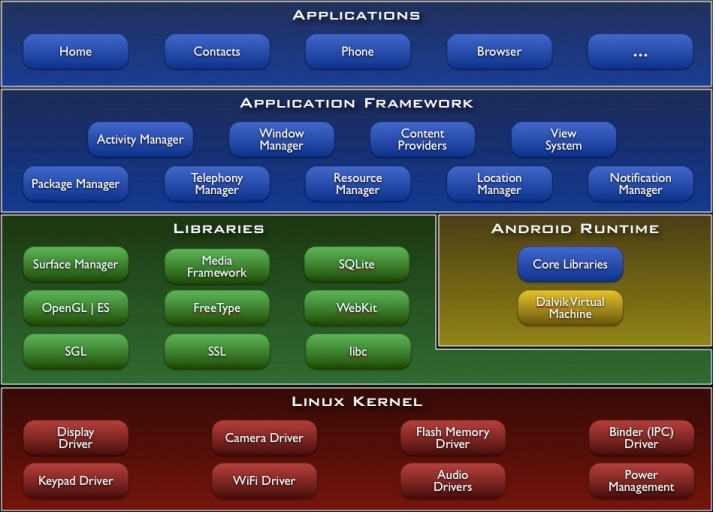
\includegraphics[width=14cm]{pics/ch1_architechture.png}
	\caption{\label{fig:ch1_architechture}Architechture du syst�me Android\protect\footnotemark}
\end{figure}
\footnotetext{\url{http://developer.android.com/guide/basics/what-is-android.html}}

\subsection{Application}
Android fournit un ensemble d'applications de bases, y compris un client email, une application SMS, un calendrier, une carte, un navigateur, etc.

\subsection{Cadre de l'application}
En fournissant une plateforme de d�veloppement ouvert, Android offre aux d�veloppeurs la possibilit� de cr�er des applications extr�mement riches et innovantes. Les d�veloppeurs sont libres de profiter du mat�riel p�riph�rique, d'obtenir les informations de la position g�ographique, d'ex�cuter les services d'arri�re-plan, d'ajouter des notifications � la barre d'�tat, etc.


Les d�veloppeurs ont un acc�s complet aux APIs utilis�s par les applications de noyau. L'architecture d'application est con�ue pour la r�utilisation des composants. 

Toutes les applications sont une collection des services, y compris : 
\bigskip
\begin{itemize}
	\item Une collection riche de \textit{View} qui peuvent �tre utilis�e pour construire une application, y compris des listes, des grilles, des zones de texte, des boutons et m�me un navigateur web � embarquer.
 	\item Des \textit{Content Providers} qui permettent aux applications d'acc�der aux donn�es provenant d'autres applications (tels que les \textit{Contacts}), ou de partager leurs donn�es.
 	\item Un \textit{Resource Manager} qui offre l'acc�s aux ressources comme les cha�nes de caract�res localis�es, les graphiques, et les fichiers de mise en page.
 	\item Un \textit{Notification Manager} qui permet toutes les applications � afficher des alertes personnalis�es dans la barre d'�tat.
 	\item Un \textit{Activity Manager} qui g�re le cycle de vie d'application et fournit une pile de navigation.
\end{itemize}

\subsection{Biblioth�ques}
Android comprend une collection de biblioth�que de C ou C++ utilis� par les composants diff�rents. Ces capacit�s sont fournies par le cadre d'application Android. Certaines de ces biblioth�ques de noyau sont montr�es ci-dessous:
\bigskip
\begin{itemize}
	\item System C library - une impl�mentation de la biblioth�que C standard du syst�me (libc).
 	\item Media Libraries - bas� sur OpenCORE de PacketVideo. Des biblioth�ques permettent l'enregistrement audio et vid�o, ainsi que des fichiers d'images, y compris MPEG4, H.264, MP3, AAC, AMR, JPG et PNG. 
 	\item Surface Manager - g�re l'acc�s au sous-syst�me d'affichage
 	\item LibWebCore - c'est un moteur de navigateur moderne qui alimente le navigateur Android et une Web View embarqu�. 
 	\item SGL - le moteur graphique 2D. 
 	\item 3D Libraries - une impl�mentation bas�e sur OpenGL ES 1.0 APIs; les biblioth�ques utilisent l'acc�l�ration mat�rielle 3D (si disponible) ou le logiciel 3D optimis� hautement.
 	\item SQLite - un moteur de base de donn�es relationnelles puissant et l�ger � la disposition pour toutes les applications.
\end{itemize}

\subsection{Phase d'ex�cution Android}
Android comprend une collection des biblioth�ques de noyau qui offrent la plupart des fonctionnalit�s disponibles du langage Java.


Chaque application Android s'ex�cute dans son propre processus, avec sa propre machine virtuelle Dalvik. Dalvik est con�ue pour qu'un mat�riel puisse ex�cuter efficacement plusieurs machines virtuelles en m�me temps. Le VM Dalvik ex�cute les fichiers de format ex�cutable Dalvik (.Dex), qui est optimis� pour la minimale d'occupation m�moire. Le VM Dalvik d�pend le noyau Linux pour les fonctionnalit�s de bas-niveau comme le management de la m�moire.

\subsection{Noyau Linux}
Android est bas� sur le noyau Linux 2.6 pour les services du syst�me noyau, tels que la s�curit�, la gestion de la m�moire, la gestion des processus, etc. Le noyau est regard� comme une couche d'abstraction entre le mat�riel et le reste de la pile logicielle.

\section{Fonctionnement des applications Android}
Toutes les applications Android sont �crites en langage Java. Les outils du SDK Android compile le code --- avec toutes les donn�es et les fichiers de ressources --- dans un package Android, un fichier d'archive avec un suffixe \textit{.apk}. Tout le code dans un seul fichier \textsl{.apk} est consid�r� comme une seule application.


Quand install� sur un mat�riel, l'application Android vit dans sa propre boite de s�curit�:
\bigskip
\begin{itemize}
	\item Le syst�me d'exploitation Android est un syst�me multi-utilisateurs, sous lequel chaque application est un utilisateur diff�rent.
 	\item Par d�faut, le syst�me attribue � chaque application un ID utilisateur Linux qui est utilis� uniquement par le syst�me et qui est inconnu pour l'application. Le syst�me d�finit les autorisations de tous les fichiers de l'application, pour que seulement les utilisateurs qui ont le droit peuvent y acc�der.
 	\item Chaque processus a sa propre machine virtuelle (VM), donc l'application fonctionne s�par�ment.
 	\item Par d�faut, chaque application s'ex�cute dans son propre processus Linux. Android d�marre le processus lorsqu'un composant de l'application doit �tre ex�cut�, et arr�te le processus quand il n'est plus n�cessaire ou quand le syst�me doit r�cup�rer la m�moire pour d'autres applications.
\end{itemize}
\bigskip

Une application Android se compose d'une collection des composants. Il y a 4 composants principaux : \textit{Activity}, \textit{Service}, \textit{ContentProvider}, \textit{BroadCast receiver}. 

\section{Environnement de d�veloppement}
%Dans cette partie, nous pr�sentons l'environnement du travail, \textcolor{red}{qui inclut les outils mat�riels et les outils de d�veloppement (logiciels et technologies exploit�s)}.


\begin{description}
	\item[Installation de JDK] \hfill \\ On d�veloppe l'application Android avec le langage Java, donc le JDK est essentiel. Dans ce projet, nous utilisons le JDK version 6, qui peut �tre t�l�charg� du site officiel\footnote{\url{http://www.oracle.com/technetwork/java/javase/downloads/index.html}}.
	
	\item[Installation de SDK Android] \hfill \\ Nous avons t�l�charg� le SDK Android depuis le site d�veloppeur Android\footnote{\url{http://developer.android.com/sdk/index.html}}. Puis, nous les avons extraits sous le r�pertoire \verb?C:\Program Files\android-sdk-windows?.
	
	\item[Installation de Eclipse] \hfill \\ Eclipse est un IDE gratuit tr�s c�l�bre dans le domaine informatique. On peut le t�l�charger � partir du site Eclipse, la version \textit{Eclipse IDE for Java Developers}est recommand�e\footnote{\url{http://www.eclipse.org/downloads/packages/eclipse-ide-java-developers/indigosr2}}.
	
	\item[Installation de ADT] \hfill \\ Dans Eclipse, cliquer par s�quence : help $\rightarrow$ Install New software $\rightarrow$ Add, puis remplir les champs en fonction de la figure\ref{fig:ch1_addrepository}:\\
		
		\begin{figure}[h]
		\centering
		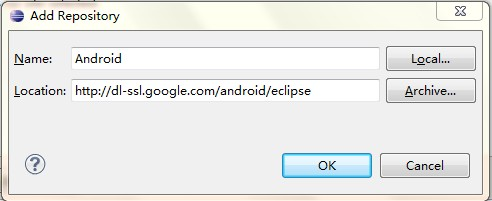
\includegraphics[width=10cm]{pics/ch1_addrepository.jpg}
		\caption{\label{fig:ch1_addrepository}Installation de ADT - Add repository}
		\end{figure}
		
		
		Apr�s cliquer sur ''OK'', Eclipse affiche les plugins disponiblies. Nous s�lectionnons le ''Android DDMS''(Android Dalvid Debug Moniter Server) et le ''ADT''(Android Development Tools). Nous validons les �tapes suivantes et nous red�marrons Eclipse pour finir l'installation des plugins. Maintenant on peut trouver les param�tre Android ici : Windows $\rightarrow$ Preferences $\rightarrow$ Android.
		
		\begin{figure}[h]
		\centering
		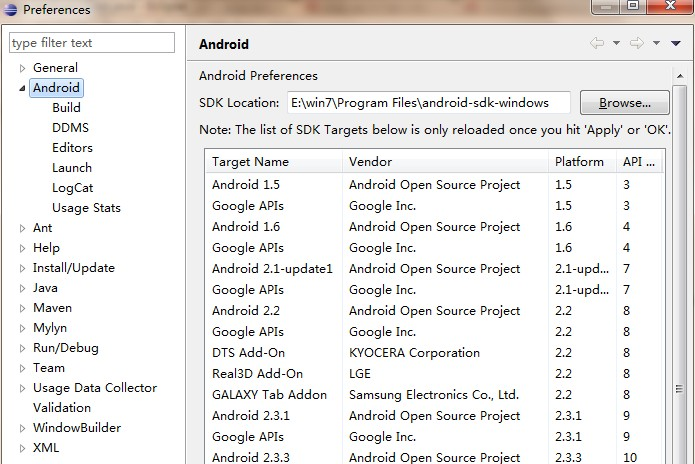
\includegraphics[width=10cm]{pics/ch1_preferences.jpg}
		\caption{\label{fig:ch1_preferences}Preferences Android}
		\end{figure}
	
	
	\item[Configuration de SDK] \hfill \\ Sous le menu Windows $\rightarrow$ Android SDK Manager, on peut s�lectionner et installer les paquets n�cessaires. Dans notre cas, API version 2.3 est suffisante. Ce qu'il faut faire attention, c'est que la version API doit �tre support� par l'appareil cibl�.
	
		\begin{figure}[h]
			\centering
			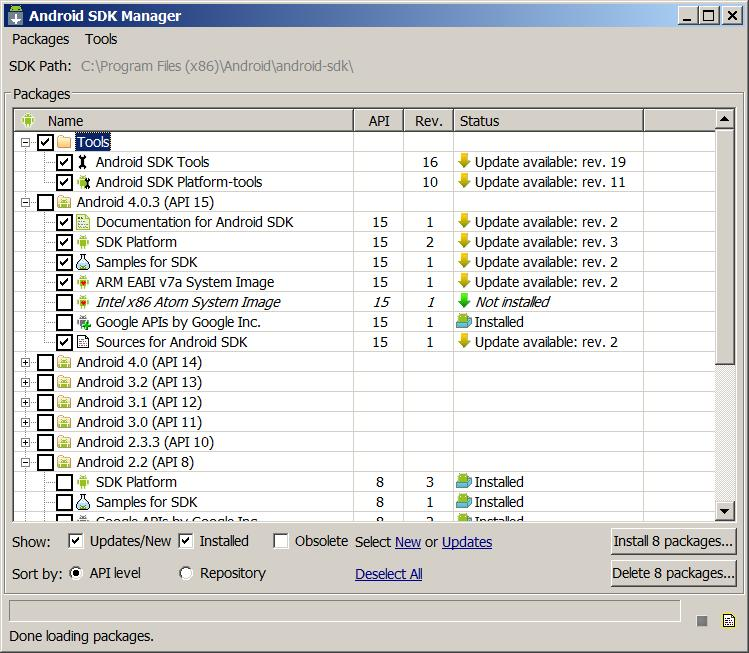
\includegraphics[width=10cm]{pics/ch1_androidsdkmanager.jpg}
			\caption{\label{fig:ch1_androidsdkmanager}Android SDK Manager}
		\end{figure}


	\item[Configuration de AVD] \hfill \\ Pour tester notre application pentant le d�veloppement, on peut utiliser directement notre portable Android, ou bien la lancer dans un appareil virtuel(AVD). Pour ce dernier, on peut lancer le gestionnaire AVD sous le menu \textit{Windows}, et cr�er un nouveau AVD en pr�cisant les param�tre. 

%\\[\intextsep]
%\begin{minipage}{\textwidth}
%\centering
%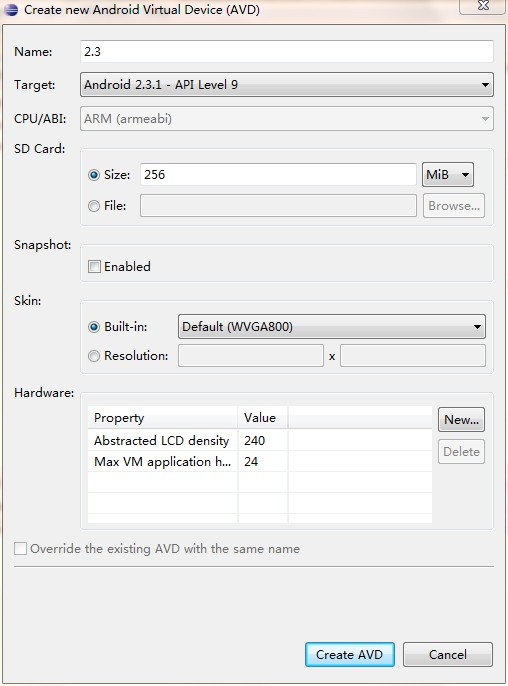
\includegraphics[width=8cm]{pics/ch1_createavd.jpg}
%\label{fig:ch1_createavd}
%\end{minipage}
%\\[\intextsep]
		\begin{figure}[!h]
			\centering
			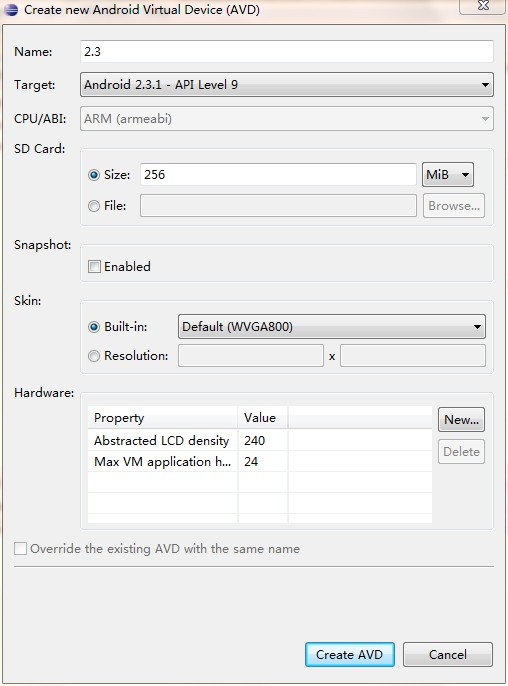
\includegraphics[width=8cm]{pics/ch1_createavd.jpg}
			\caption{\label{fig:ch1_createavd}Cr�ation d'un AVD}
		\end{figure}


\end{description}

\chapter{Carte AndroPOD}
\section{Introduction}
L'Interface AndroPOD sert d'un port s�rie pour les t�l�phones ou les tablettes Android. Il fonctionne avec l'appareil Android non modifi�. Contrairement � toutes les autres solutions similaires sur le march�, l'interface AndroPOD permet les d�veloppeurs pour d�boguer l'application de t�l�phone lorsque le t�l�phone est connect� � l'interface AndroPOD. Donc c'est un outil qui peut beaucoup faciliter le d�veloppement des applications Android.


Deux acticles\footnote{\url{http://www.elektor.fr/magazines/2012/fevrier/andropod-(1).2057762.lynkx}} \footnote{\url{http://www.elektor.fr/magazines/2012/mars/andropod-(2).2085663.lynkx}} provenant du magazine \textit{Elector} introduisent en d�tail la fonctionnalit� de la carte avec un exemple r�alis�. La carte �tait aussi command�e sur ce site.


L'interface AndroPOD est con�ue pour �tre int�gr� dans votre propre projet. Nous pouvons l'utiliser dans plusieurs situations, par exemple pour les robots, les gadgets ou tous autres projets qu'on peut penser. Avec l'interface AndroPOD, on renforce son projet avec les fonctionnalit�s WIFI, 3G, 4G, Bluetooth, GPS etc. Si on a besoin un grand �cran couleur avec �cran tactile, AndroPOD peut aussi offre ses aides. Dans notre projet, nous l'utilisons pour que l'on puisse contr�ler le robot Lynxmotion avec notre appareil\footnote{Samsung Galaxy Nexus, fourni par l'�cole} Android.

\section{Utilisation}

Sur ce site\footnote{\url{http://www.xdevelop.at}}, nous avons trouv� un tutorial d�tail� pour prendre en mains AndroPOD. 


Pour connecter et communiquer avec la carte � partir du bout Android, il suffit d'�tablir un serveur TCP sur le port 1337.


\begin{lstlisting}
try
{
     //Etablir un serveur sur le port 1337
     ServerSocket socket = new ServerSocket(1337);
    
     //Attendre la connexion de Andropod
     Socket andropodInterface = socket.accept();

     //Ouvrir IO flux
     PrintReader in = new BufferedReader(new InputStreamReader(andropodInterface.getInputStream()));
     PrintWriter out = new PrintWriter(andropodInterface.getOutputStream(), true);

     //Envoyer ce que vous voulez
     out.println("Hello Androdpod!");

     //Recevoir les donn�es
     string message = in.readln();
}
catch (IOException e) 
{
     //En cas d'exception
} 
\end{lstlisting}


D'autre part, pour relier AndroPOD et le mobile avec le c�ble usb-microusb fourni, il suffit de faire apr�s ces 5 �tapes :
\bigskip
\begin{enumerate}
	\item \textbf{Configuration de l'interface Andropod avec le PC}\\
Installer le logiciel de configuration Andropod sur le PC, changer l'interface Andropod en ''Configure mode'' (voir figure\ref{fig:ch2_carte}) et la connecter au PC en utilisant un USB c�ble. Ensuite, on peut �ventuellement configurer les autres param�tres avec \textit{AndroPOD Interface Controller}(figure\ref{fig:ch2_andropodcontroller}).

\begin{figure}[!ht]
	\centering
		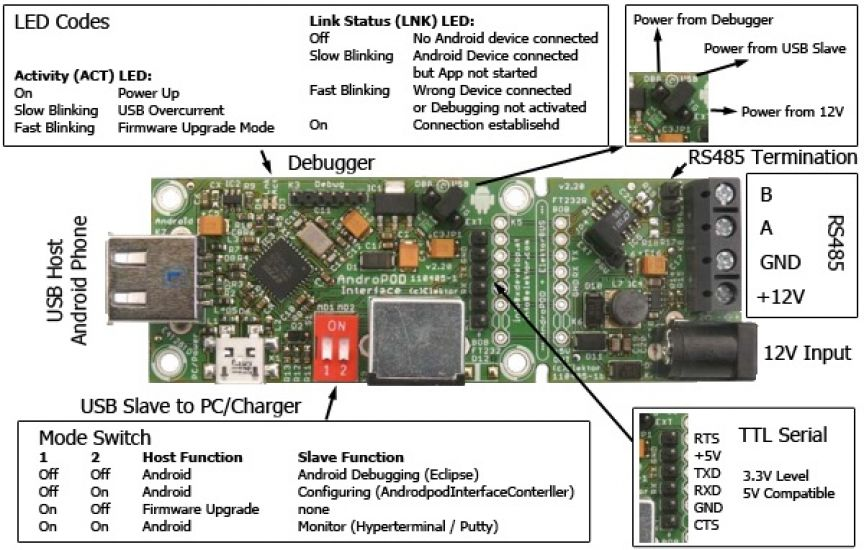
\includegraphics[width=14cm]{pics/ch2_carte.jpg}
	\caption{La carte AndroPOD}
	\label{fig:ch2_carte}
\end{figure}

\begin{figure}[!ht]
	\centering
		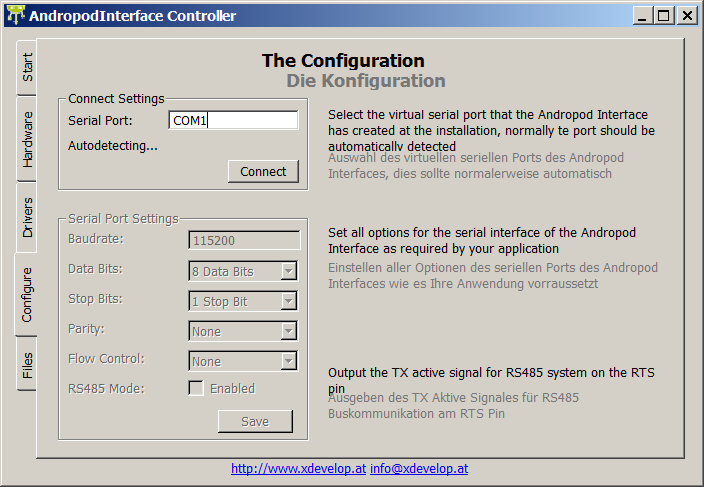
\includegraphics[width=14cm]{pics/ch2_andropodcontroller.png}
	\caption{AndroPOD Interface Controller}
	\label{fig:ch2_andropodcontroller}
\end{figure}

	\item \textbf{Connecter-la au robot}\\
Utiliser quatre fils simples, dont deux pour le voltage +5 V, GND et les deux autres pour RX et TX. L'interface AndroPOD a besoin de 5V vers 550mA afin de charger le t�l�phone Android (si on n'arrive pas � charger le t�l�phone lorsqu'il est connect� � l'USB , l'�nergie sera consomm�e tr�s vite. C'est notre cas.). Maintenant une LED sur l'interface Andropod doit s'allumer.

	\item \textbf{Activer l'option ''D�bogage USB'' sur le mobile Android}\\

	\item \textbf{Connectez l'appareil Android � Andropod}\\
Maintenant la deuxi�me LED sur l'interface AndroPOD devrait commencer � clignoter, et le t�l�phone devrait nous dire que le d�bogage USB est connect�.

	\item \textbf{D�marrez l'application sur le t�l�phone Android}
Maintenant la deuxi�me LED arr�te de clignoter et rester allum�e.
\end{enumerate}


Apr�s ces 5 �tapes, nous avons r�ussi de connecter l'interface AndroPOD.




\begin{figure}[!ht]
	\centering
		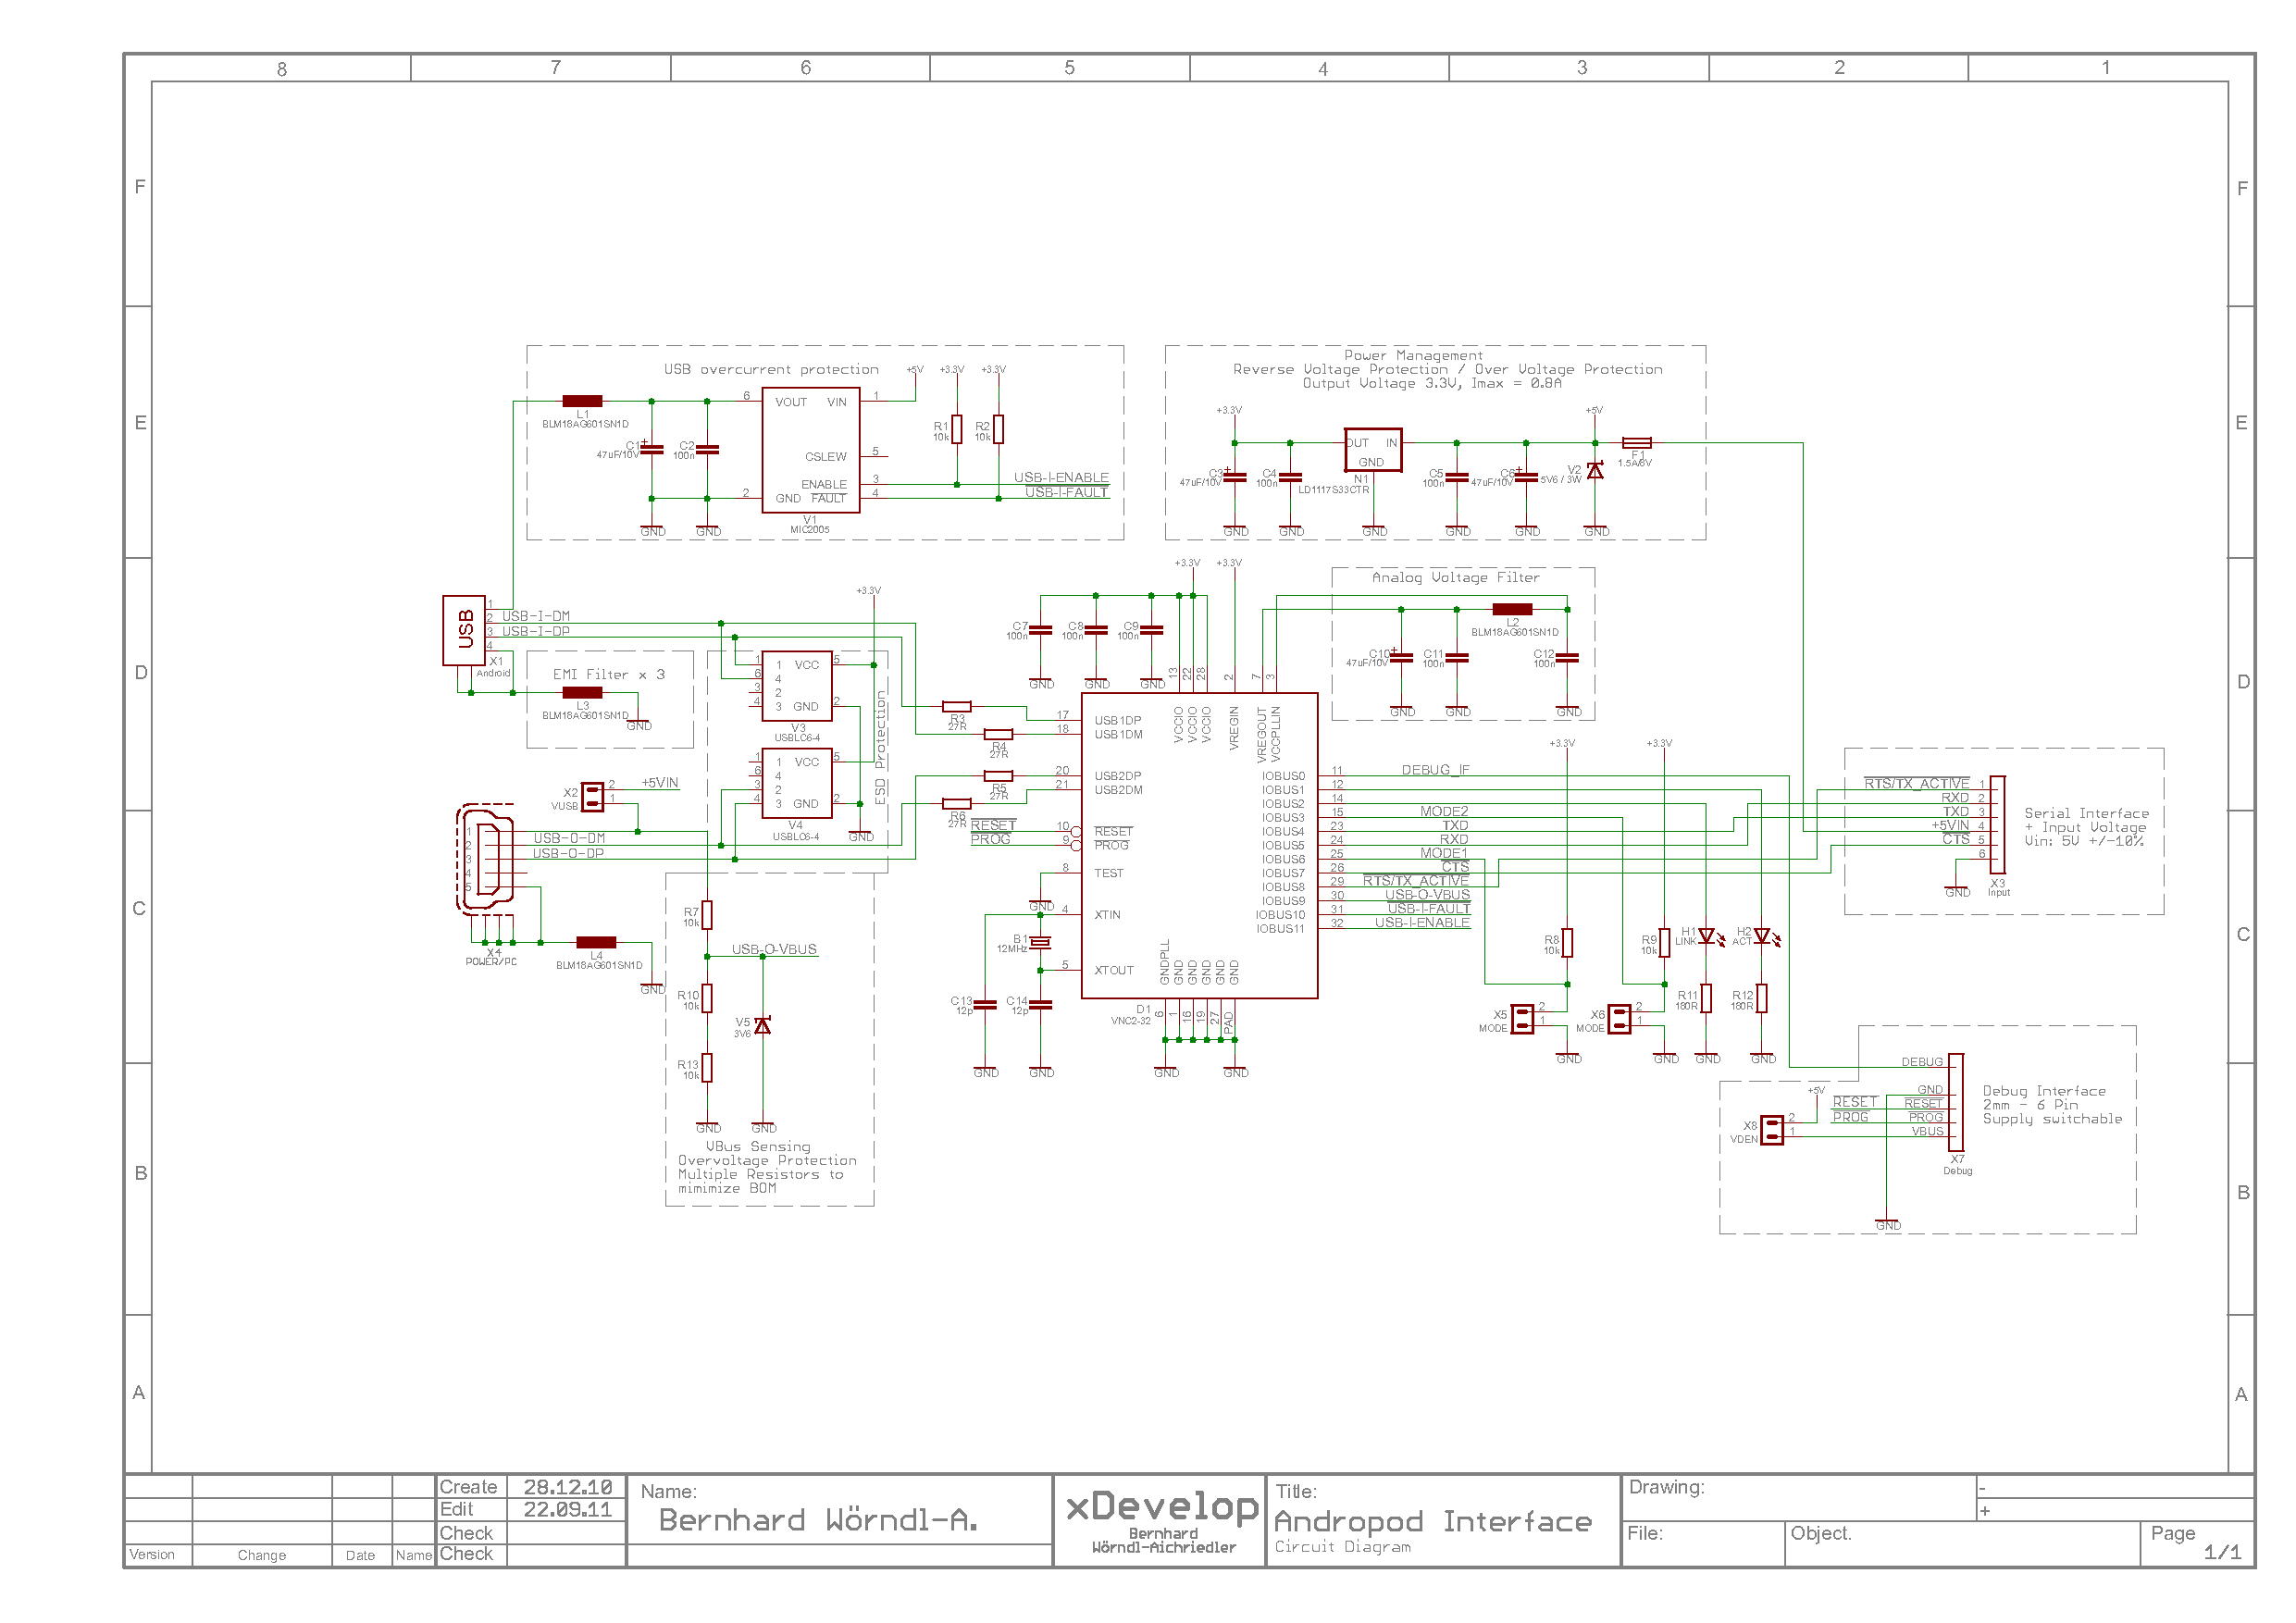
\includegraphics[width=16cm]{pics/ch2_schema.pdf}
	\caption{Sch�ma de la carte AndroPOD}
	\label{fig:ch2_schema}
\end{figure}

\chapter{Robot Lynxmotion}
\section{Introduction}
Nous choisissons le robot Lynxmotion comme le mat�riel � contr�ler par AndroPOD, parce qu'il n'existe actuellement pas beaucoup d'�quipement qui se munit encore une interface s�rie dont AndroPOD a besoin pour le contr�ler. D'ailleurs, contr�ler un petit robot avec un mobile est une fa�on assez directe pour montrer la force de la carte AndroPOD.
\begin{figure}[!ht]
	\centering
		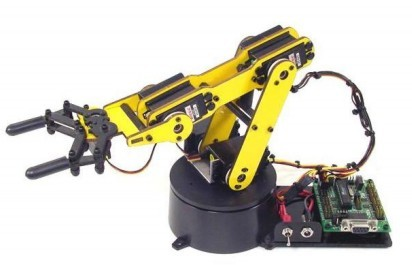
\includegraphics[width=14cm]{pics/ch3_robot.jpg}
	\caption{Robot Lynxmotion}
	\label{fig:ch3_robot}
\end{figure}

Le robot est un bras robotis� dont les documentations sont disponibles sur le site de Lynxmotion\footnote{\url{http://www.lynxmotion.com/driver.aspx?Topic=assem01\#l6}}. Il a �t� utilis� avant dans un notre projet, alors tout d'abord nous essayons de v�rifier son �tat de fonctionnement. Nous avons install� son logiciel de contr�le nomm� \textit{LynxTerm} qui a une interface comme figure\ref{fig:ch3_lynxterm}. Pour faire fonctionner ce logiciel, il faut que l'on installe un pilote USB-to-Serial\footnote{\url{http://www.prolific.com.tw/eng/downloads.asp?id=31}}, pour avoir un port s�rie virtuel.
\begin{figure}[!ht]
	\centering
		\includegraphics[width=14cm]{pics/ch3_lynxterm.jpg}
	\caption{Terminal de contr�le : LynxTerm}
	\label{fig:ch3_lynxterm}
\end{figure}

Avec ce logiciel de contr�le, nous avons trouv� qu'il y a 5 servomoteurs au total dont 2 ne fonctionnent pas, mais nous ne les avons pas puisque �a ne nous emp�che pas de montrer la fonctionnalit� de l'AndroPOD. Alors maintenant, ce qui nous int�resse, c'est le format de commandes pour contr�ler ce robot, c'est-�-dire les informations transmises entre LynxTerm et le robot.

\section{Format des commandes}
Pour trouver la structure des commandes, nous avons �tudi� le manuel de r�f�rence de la carte SSC-32\footnote{Il est attach� � la fin du rapport. On peut le trouver aussi ici : \url{http://www.lynxmotion.com/images/data/ssc-32.pdf}} qui est int�gr� avec le robot, et qui re�ois et traite les commandes. Finalement, nous constatons que le format de commandes est de forme ''\# <ch> P <pw> S <spd> T<time> <cr>'', dont les explications sont :
\bigskip
\begin{itemize}
	\item <ch> : Le num�ro de canal, forme d�cimal, 0-31. Il correspond au servomoteur qu'on veut contr�ler ;
 	\item <pw> : La largeur de pulsation en microseconde, 500-2500 ;
 	\item <spd> (facultatif) : La vitesse de mouvement en microseconde ; 
 	\item <time> (facultatif) : La dur�e en milliseconde d�sign�e pour un mouvement complet, valide pour tous les canaux ;
 	\item <cr> : Retour de chariot, ASCII 13, obligatoire pour finir une commande.
\end{itemize}
\bigskip


Dans les commandes au-dessus, il y a des param�tres en microseconde qui concernent � la conception au moteur servo. Puisque c'est un peu loin de notre but du projet, on ne va pas �tudier profond�ment sur ce point, par contre il suffit de savoir la position en angle correspondante comme l'indiqu� � la figure\ref{fig:ch3_motorrange}.
\begin{figure}[!ht]
	\centering
		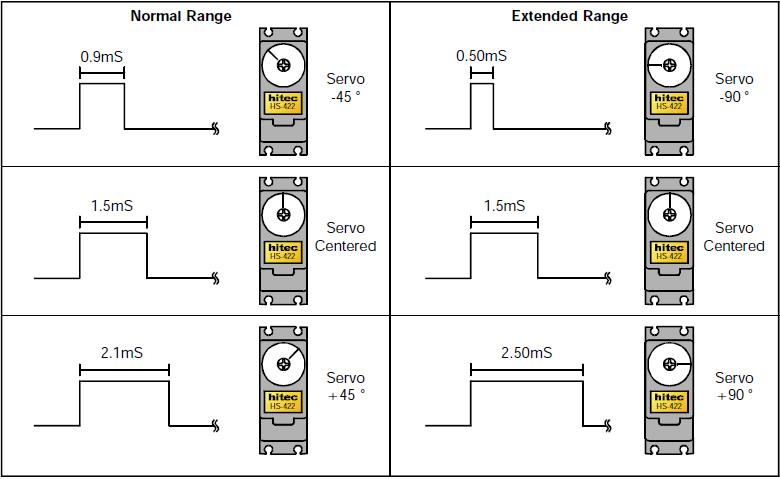
\includegraphics[width=14cm]{pics/ch3_motorrange.jpg}
	\caption{Mouvement des servomoteurs du robot}
	\label{fig:ch3_motorrange}
\end{figure}

Maintenant on conna�t le format de commandes. Par exemple, la commande \textit{\#5 P1500 S100 <cr>} d�place le moteur 5 � la position centrale (2\ieme{} rang�e dans la figure\ref{fig:ch3_motorrange}), ayant une vitesse de 100$\mu$s par seconde. Un mouvement de 1000$\mu$s correspond au $90^\circ$, donc ''100$\mu$s par seconde'' signifie que �a co�te 10 secondes � tourner $90^\circ$.

\begin{figure}[!ht]
	\centering
		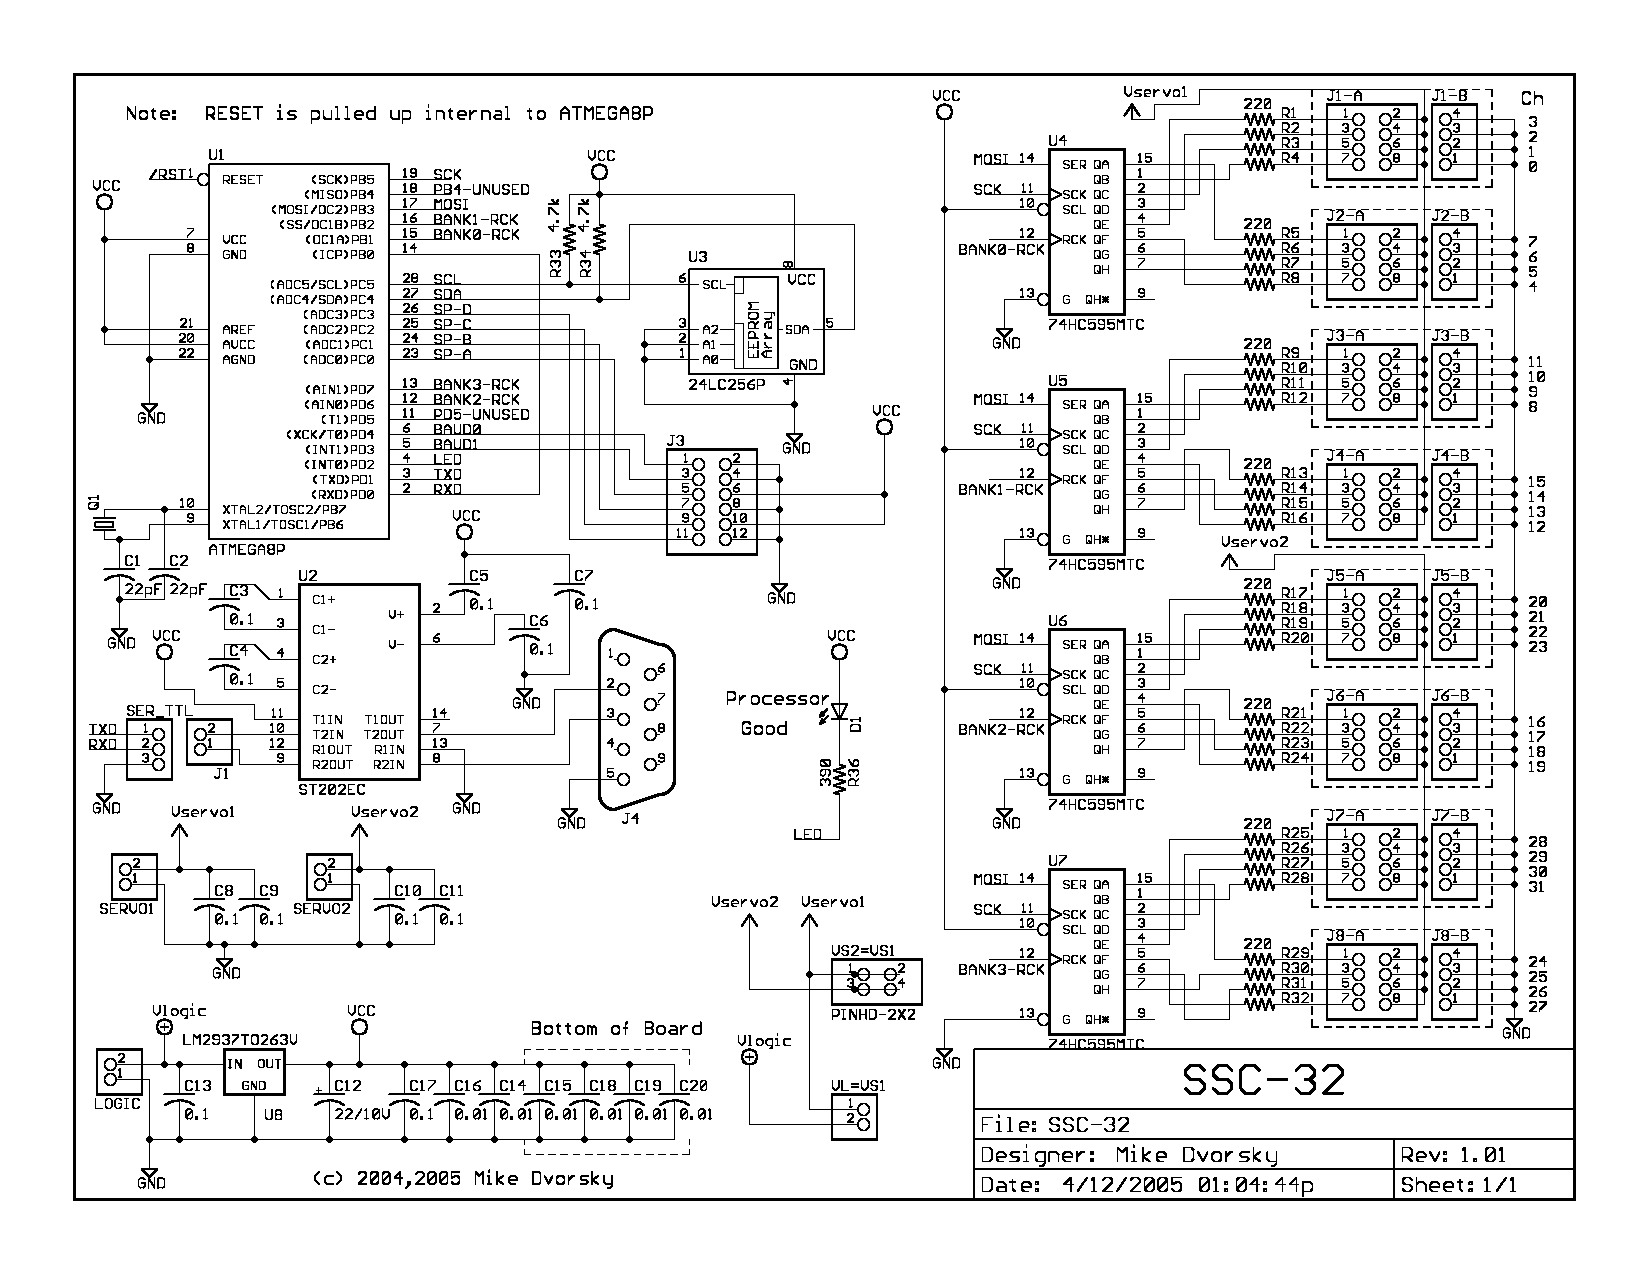
\includegraphics[width=16cm]{pics/ch3_schema_ssc32.pdf}
	\caption{Sch�ma de la carte SSC32 int�gr�e avec le robot}
	\label{fig:ch3_schema_ssc32}
\end{figure}

\chapter{Mise en oeuvre}
%mise en oeuvre
Sur le site\footnote{\url{http://www.xdevelop.at}}, il y a des tutoriaux assez d�taill�s pour commence � programmer pour AndroPOD. Ils offrent m�me un petit projet d'exemple qui a une fonctionnalite �l�mentaire pour communiquer entre l'application et AndroPOD par la connexion TCP. Ayant auparavant des connaissances sur Java et la programmation des r�seaux, nous avons �tudi� ce petit programme qui a facilit� notre travail.


Notre application poss�de une interface ci-dessous \ref{fig:ch4_interface}:

\begin{figure}[!ht]
\centering
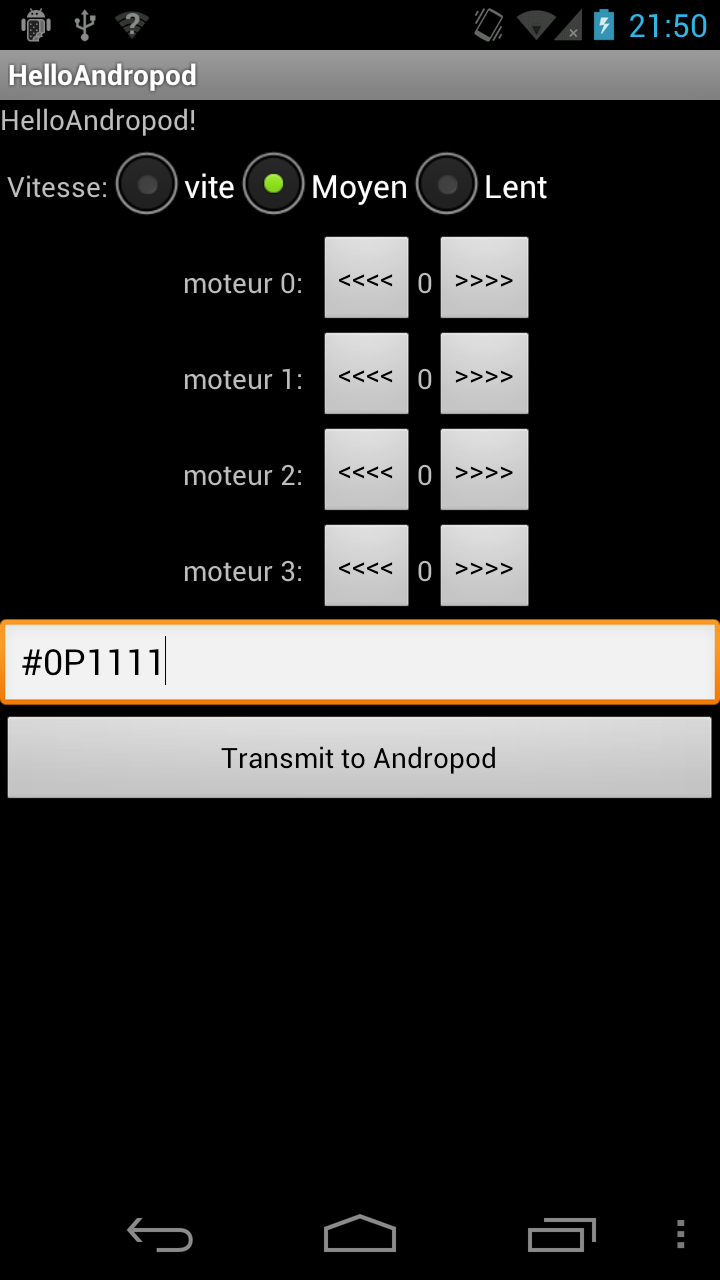
\includegraphics[width=6cm]{pics/ch4_interface.png}%
\caption{L'interface de l'application}%
\label{fig:ch4_interface}%
\end{figure}
%\\[\intextsep]
%\begin{minipage}{\textwidth}
%\centering
%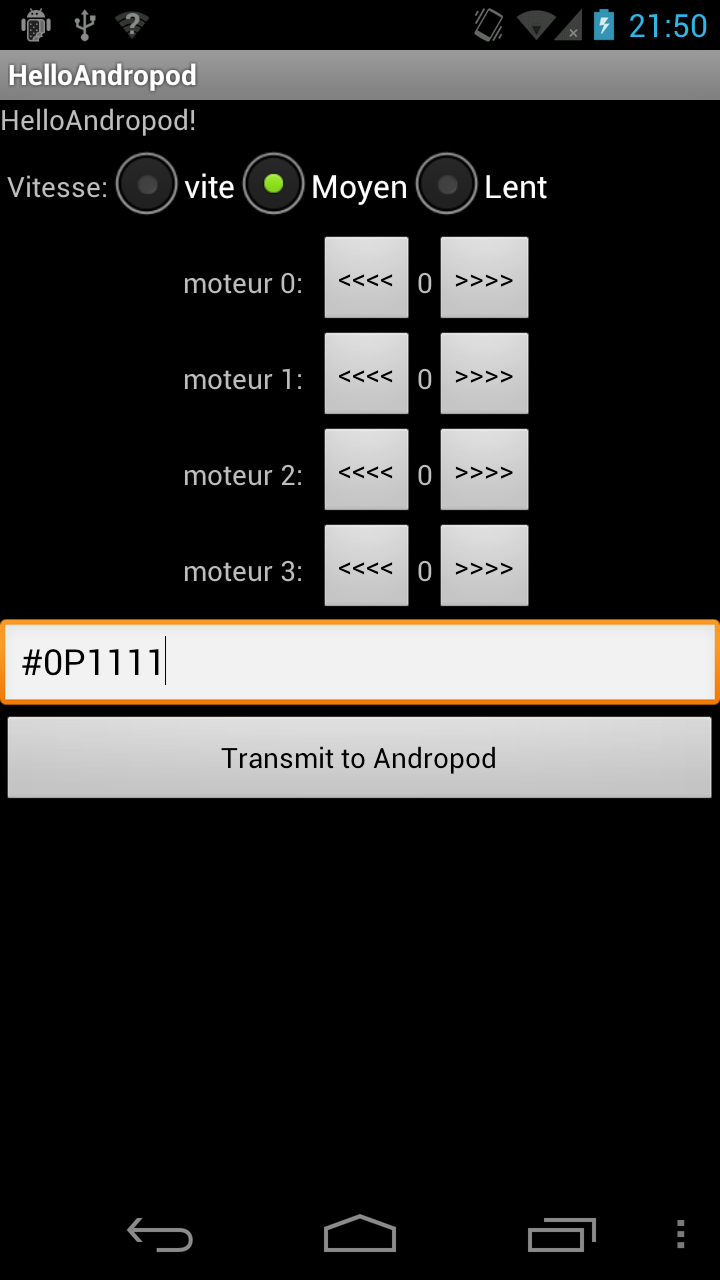
\includegraphics[width=5cm]{pics/ch4_interface.png}
%\label{fig:ch4_interface}
%\end{minipage}
%\\[\intextsep]

A la fin, nous avons reli� toutes les trois parties --- mobile, AndroPOD et ordinateur, et nous avons r�ussit de contr�ler le robot avec notre mobile.

\begin{figure}[!ht]
\centering
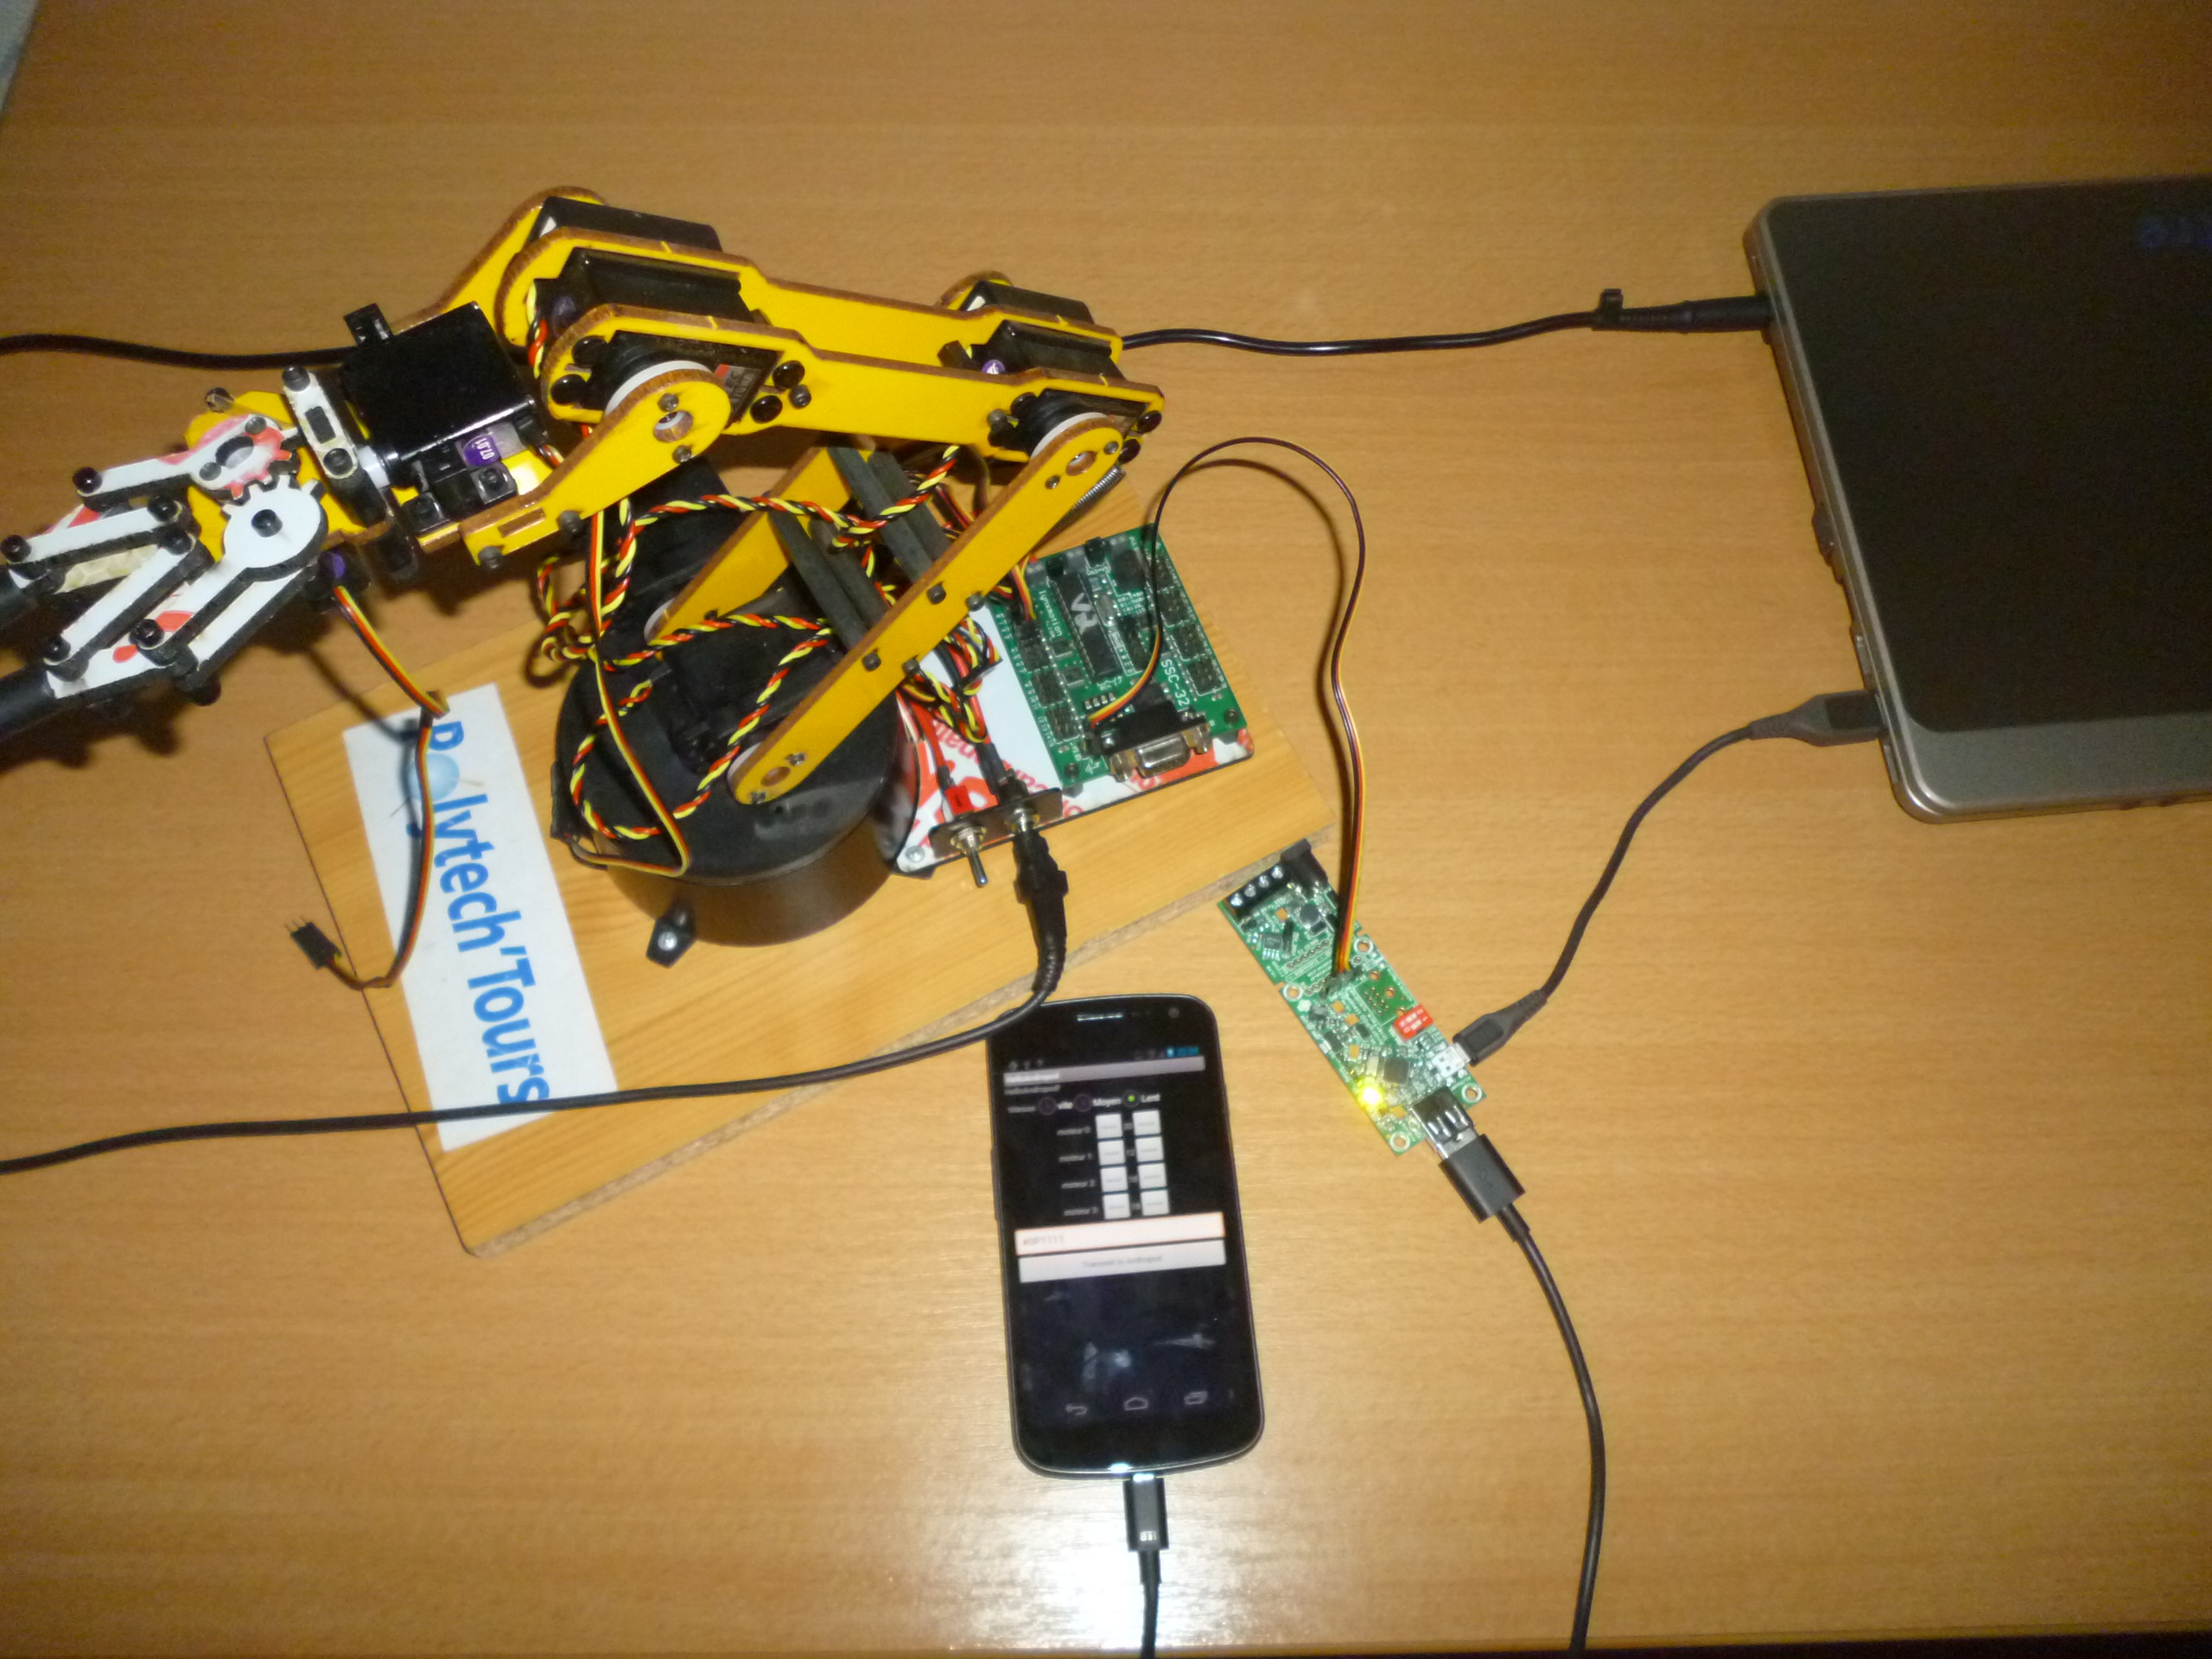
\includegraphics[width=14cm]{pics/ch4_ensemble.JPG}%
\caption{L'oeuvre finale}%
\label{fig:ch4_ensemble}%
\end{figure}

\chapter{Difficult�s rencontr�es}
Pendant le d�veloppement de ce projet, nous avons rencontr� quelques difficult�s :
\begin{description}
	\item[D�veloppement sous Android] \hfill \\
Puisque Android est inconnu pour nous, c'est une grande difficult�. Pour le conqu�rir, nous avons pas d'autre choix sauf d�penser beaucoup de temps � lire les acticles r�ferents, surtout les documentations du site de d�veloppeurs d'Android. Notre application ne n�cessite que une connaissance base sur Android, donc apr�s une p�riode d'�tude, nous avons matris� les connaissances n�cessaires pour r�aliser notre application.

	\item[Connaissance du robot] \hfill \\
Quand nous avons re�u le robot, nous ne connaissions pas vraiment c'est quoi un robot, et comment le contr�ler. Alors M. Makris nous avons donn� un rapport d'un projet avant sur ce robot , et apr�s la lecture, nous avons eu une connaissance compl�te.

	\item[Connextion entre AndroPOD et le robot] \hfill \\
Le robot a une interface s�rie RS232 mais celle d'AndroPOD est une interface TTL. Au d�but nous avons pens� que l'on peut connecter directement les deux port, parce que la RS232 contient aussi les 3 boches TX,RX,GND, qui composent la TTL. Mais �a n'a pas march�. Par hasard, nous avons trouv� qu'il existe aussi une interface TTL sur la carte du robot ! Alors nous l'avons v�rifi�s et l'essay�s, par cons�quent, nous avons r�ussi.

	\item[Recherche du format de commands] \hfill \\
Au d�but, c'�tait difficile pour nous � savoir le vrai format de commands transmis, et nous devions absolument le savoir pour cr�er notre propre application. M�me si on peut trouver des information sur le manuel d'utilisateur de la carte ssc-32 int�gr�e avec le robot, on veut toujour savoir exactement ce qui se passe. Enfin nous avons trouv� un logiel qui peut surveiller les vraies donn�es transmis par le port s�rie de \textit{LynxTerm} au robot, et donc nous avons r�solus ce probl�me.

	\item[R�daction du rapport] \hfill \\
Cette difficult� est en fait � cause de notre niveau du fran�ais. M�me si nous avons d�j� �tudi� la langue il y a presque un an, c'est quand m�me probl�matique de r�diger un rapport en fran�ais. Mais c'est aussi, pour nous, une chance de pratique la langue.
\end{description}


Pour faire un r�sum�, il y a deux raisons pourquoi nous avons enfin pu trouv� les solution. D'une part, nous avons pris fr�quemment des rendez-vous avec M. Makris, qui nous a renseign� beaucoup; d'autre part, nous avons pu trouv� beaucoup de documentations outils, et nous les avons bien lus.

\chapter{Conclusion}
Notre projet contient trois parties principales : le syst�me Android, la carte AndroPOD et le petit robot. Nous avons fait beaucoup de recherche et d'�tude pour connaitre chacune partie, et � la fin de notre projet, nous avons r�ussi � contr�ler le robot avec notre mobile Android, ayant AndroPOD comme le pont entre eux, et une application install�e sur le mobile.


La programmation sous Android est en vogue pour le moment. Ce projet nous permet pas seulement d'avoir une connaissance fondamentale du d�veloppement sous Android, mais encore d'avoir une impression sur le contr�le de mat�riel. C'est aussi int�ressant de faire un lien entre notre mobile Android et un petit robot. 
A la fin, nous voudrions remercier notre encadrant M. Pascal Makris, qui nous a accompagn� tout au long du d�veloppement du projet, en nous guidant par les r�unions fr�quentes et en nous offrant les mat�riels requis.


\annexes

\end{document}

